%ustawienia
\documentclass[12pt,a4paper]{article}
\usepackage[T1]{fontenc}
\usepackage{mathptmx}
\usepackage[utf8]{inputenc}
\usepackage{amssymb}
\usepackage[polish]{babel}
\usepackage{polski}
\usepackage{amsmath}
\usepackage{amsfonts}
\usepackage[left=3.5cm,right=2cm,top=2.5cm,bottom=2.5cm]{geometry}
\usepackage{graphicx}
\usepackage{indentfirst} 
\usepackage{float}
\usepackage{hyperref}
\usepackage[most]{tcolorbox}
\setlength{\parindent}{0.7cm}
\hypersetup{
	colorlinks = true,
	linkcolor = black,
	filecolor = magenta,
	urlcolor = blue,
	}
\urlstyle{same}	
	
\author{Projektowanie i wdrażanie systemów informatycznych\\\\\\\\\\\\\includegraphics[width=0.7\linewidth]{img/logoPWSZ.eps}\\\\\\\\Karpiński Maciej\\Krysa Marcin\\Kuczma Łukasz\\Mertuszka Adam\\\\\\\\}
\title{}

\begin{document}

	%Stron tytułowa
	\maketitle
	\thispagestyle{empty}
	\pagenumbering{arabic} 
	\clearpage

	%Spis treści
	\tableofcontents
	\newpage

	%Psekcja pierwsza, opisująca firmę
	\section{Prezentacja firmy}
		\indent Opis firmy
	\newpage

	%sekcja druga, Analiza słabych, mocnych, szans i zagrożenia 
	\section{Analiza SWOT}
		\indent Analiza SWOT
	\newpage
	
	%Sekcja trzecia, analiza potrzeb
	\section{Analiza potrzeb informacyjnych}
		\indent Lider projektu Adam Mertuszka jest jednocześnie pracownikiem firmy, posiada wiedzę dotyczącą procedur i obiegu dokumentów w firmie. Celem projektowanego systemu
			informatycznego jest usprawnienie realizacji umów z~kontrahentami poprzez poprawę obiegu dokumentów oraz skuteczne gromadzenie informacji na temat zamówienia, tak aby dział
			realizujący zamówienie posiadał kompletną listę zamówionych elementów i inny rzeczy wymaganych do montażu u klienta, bez konieczności
			przeglądania umów przez pracownika magazynu w dziale sprzedaży. Model działania systemu informatycznego przedstawia rysunek nr. \ref{fig:sys_model}\\
			\begin{figure}[H]
			\centering
			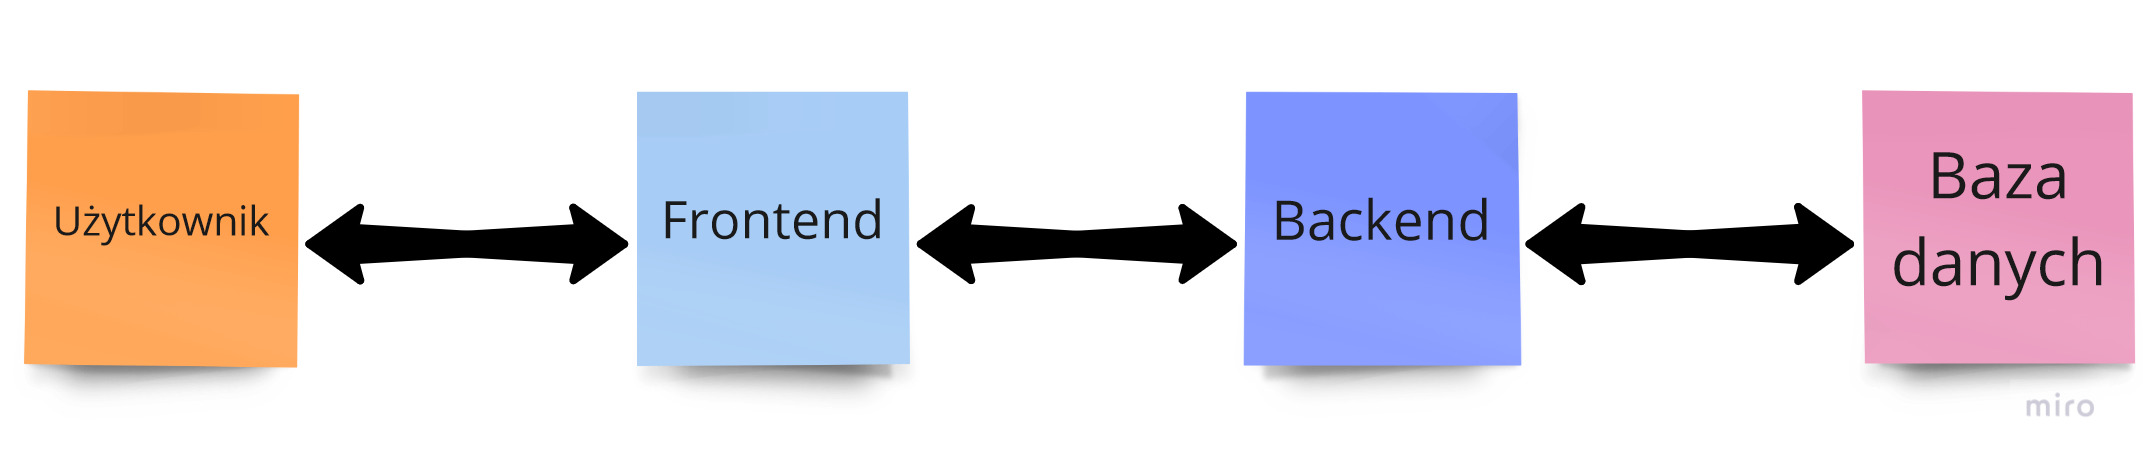
\includegraphics[width=\textwidth]{img/model_systemu_informatycznego.jpg}
			\caption{Model systemu infromatycznego}
			\label{fig:sys_model}
		\end{figure}
		\indent Dobór oraz zakup oprogramowania i podzespołów komputerowych, na którym będzie funkcjonował system informatyczny. \\ 
		\indent Dostosowanie infrastruktury sieciowej - rozszerzenie i konfiguracja dotychczas istniejącej infrastruktury sieciowej o możliwość podłączenia serwera udostępniającego
			system informatyczny.\\		
		\indent System informatyczny składa się z trzech głównych modułów tj:
			\begin{itemize}
				\item Backend - API
				\item Baza danych
				\item Frontend
			\end{itemize}
		\indent Backend - API, realizuje łączność między modułem frontendu a bazą danych, jest odpowiedzialny za przetwarzanie i udostępnianie danych. Backend udostępnia API
			dzięki, któremu	moduł frontendu ma możliwość pobierania i wysyłania niezbędnych danych z bazy danych. Zastosowanie API pozwala w przyszłości rozbudować system o nową
			funkcjonalność lub alternatywne moduły komunikacyjne z użytkownikiem. Budowa backendu uniemożliwia pobieranie zbędnych danych, dzięki czemu ruch sieciowy oraz wymagana moc
			obliczeniowa jest ograniczona do niezbędnego minimum. Rysunek nr. \ref{fig:api_model} przedstawia model budowy Backendu - API.\\
		\begin{figure}[h]
			\centering
			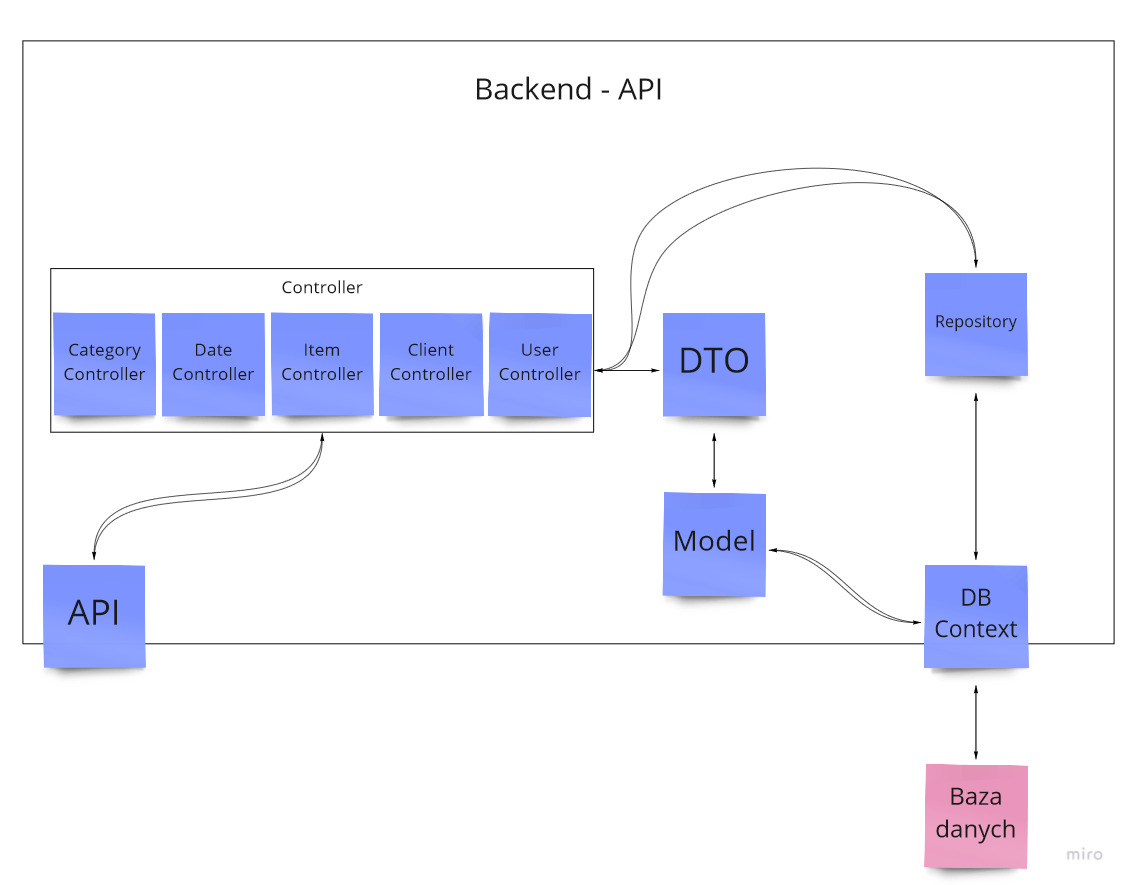
\includegraphics[width=\textwidth]{img/Backend-API_model.jpg}
			\caption{Model Backend - API}
			\label{fig:api_model}
		\end{figure}
		\indent Baza danych realizuje funkcję gromadzenia danych wprowadzanych przez użytkowników. Dane wprowadzone do bazy danych są raz dziennie automatycznie archiwizowane
			w kopii zapasowej na twardym dysku zgodnie z ustawionym harmonogramem. Model bazy danych przedstawia rysunek nr. \ref{fig:db_model}\\
		\begin{figure}[H]
			\centering
			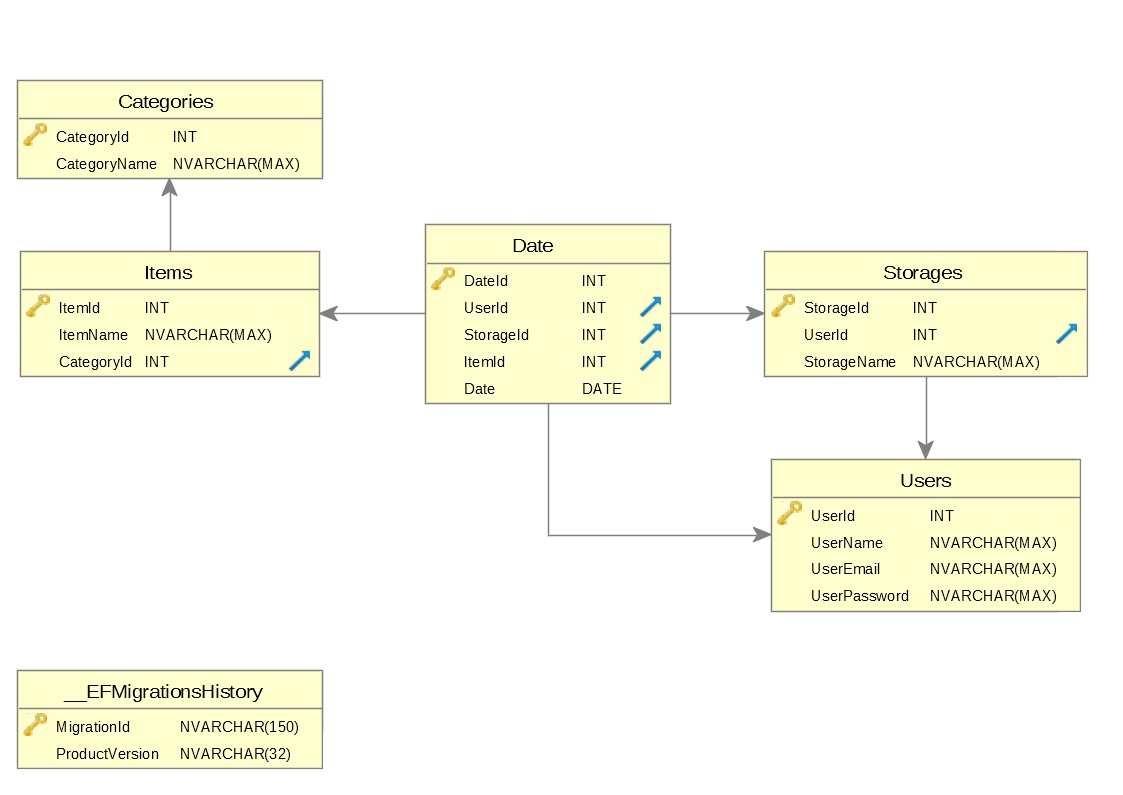
\includegraphics[width=0.9\textwidth]{img/model_bazy_danych.jpg}
			\caption{Model bazy danych}
		\label{fig:db_model}
		\end{figure}
		\indent Frontend realizuje funkcje komunikacji pomiędzy użytkownikiem a modułem backendu. Udostępnia prosty i przejrzysty interfejs użytkownika, przetwarza
			dane pobrane z API w sposób przyjazny dla użytkownika, oraz umożliwia w łatwy sposób wprowadzanie nowych danych do systemu informatycznego.\\			  
		\indent System informacyjny realizuje następującą funkcjonalność:
			\begin{itemize}
				\item Przyjazny interfejs użytkownika - interfejs użytkownika był projektowany i konsultowany wraz z użytkownikami przedsiębiorstwa, którzy będą go codziennie
					wykorzystywać do pracy;
				\item Tworzenie i logowanie użytkowników systemu - po otworzeniu okna systemu informatycznego użytkownik będzie miał możliwość zalogowania się na swoje indywidualne konto
					lub w przypadku nowego użytkownika jego utworzenie;
				\item Nadawanie uprawnień użytkownikom - administrator systemu może przypisywać uprawnienia dla kont użytkowników, ograniczając im funkcjonalność jedynie do niezbędnych
					przy wykonywaniu pracy; 
				\item Użytkownik działu sprzedaży może tworzyć i modyfikować ,,kontener'' zawierający listę zamówień, numer umowy oraz termin i adres realizacji zamówienia;
				\item Użytkownik działu magazynowego może przeglądać listę utworzonych ,,kontenerów'' dzięki czemu będzie mógł uzupełnić magazyn o brakujące elementy;
				\item Użytkownik działu realizacji zamówienia może przeglądać listę utworzonych ,,kontenerów'' dzięki czemu wie kiedy i gdzie będzie musiał przystąpić do realizacji zamówienia;
				\item Logowanie akcji użytkowników - system informatyczny loguje wszystkie podejmowane przez użytkowników akcje. Administrator posiada możliwość przeglądania
					wygenerowanych logów, dzięki czemu ma wgląd w działanie systemu informatycznego;  
				\item Zabezpieczenie przed utratą danych - system operacyjny serwera został skonfigurowany w taki sposób aby była automatycznie tworzona kopia zapasowa danych,
					kontrola jej integralności oraz aby możliwe było odtworzenie stanu sprzed awarii maksymalnie jednego twardego dysku.
					Funkcja realizująca archiwizację danych uruchamia się automatycznie codziennie o godzinie 19:00 oraz powinna zakończyć się maksymalnie o godzinie 5:00, pozostałe funkcje
					zabezpieczające działają ciągle w tle jako część systemu plików i macierzy RAID-Z;
				\item Zabezpieczenie przed nieautoryzowanym dostępem do danych - dostęp do systemu informatycznego wymaga logowania, wszystkie dane przesyłane pomiędzy systemem informatycznym
					a użytkownikiem są szyfrowane asynchronicznie. Dostęp do serwera wymaga autoryzacji, konto ,,root'' wymaga podania specjalnego hasła, wszystkie dane na dysku
					są automatycznie szyfrowane. Dostęp do bazy danych wymaga autoryzacji, system nie jest dostępny poprzez sieć internetową - działa jedynie w lokalnej sieci Ethernet.
					Zapora sieciowa na serwerze automatycznie blokuje wszelki ruch na portach, które nie są wykorzystywane w realizacji zadań systemu informatycznego, systemu operacyjnego
					oraz usługi konteneryzacji Docker;
			\end{itemize}
		\indent System informatyczny musi działać na wszystkich komputerach znajdujących się w firmie - zrealizowane jest to dzięki zrealizowaniu frontendu systemu jako aplikacji
				webowej, która do uruchomienia wymaga jedynie współczesnej przeglądarki internetowej.		
	\newpage
	
	%Sekcja czawarta, wybór narzędzi
	\section{Wybór narzędzi}
		\subsection{ASP.NET Core 3.1}
			\indent ASP.Net Core jest wysokowydajnym frameworkiem, do budowania nowoczesnych aplikacji internetowych wykorzystujących moc obliczeniową chmur. ASP.Net Core jest technologią
			open - source, wykorzystującą silnik html Razor, dzięki której możliwe jest tworzenie aplikacji mulitplaformowych, które mogą być używane na każdym urządzeniu wyposażonym
			w przeglądarkę internetową.

		\subsection{AutoMapper}
			\indent AutoMapper jest biblioteką służącą do mapowania między obiektami, dzięki czemu można automatycznie mapować właściwości dwóch różnych obiektów,
					przekształcając obiekt wejściowy jednego typu na obiekt wyjściowy innego typu.  
		\subsection{C\#}
			\indent C\# jest obiektowym językiem programowania, zaprojektowanym w latach 1998 – 2001 dla firmy Microsoft.
			Napisany program jest kompilowany do Common Intermediate Language(CLI), który następnie wykonywany jest w środowisku uruchomieniowym takim jak .NET Framework,
			.NET Core, Mono lub DotGNU.
			Wykorzystanie CLI sprawia, że kod programu jest wieleplatformowy (dopóki istnieje odpowiednie środowisko uruchomieniowe).
			C\# posiada wiele wspólnych cech z językami Object Pascal, Delphi, C++ i Java a najważniejszymi cechami C\# są:
			\begin{itemize}
				\item Obiektowość z hierarchią o jednym elemencie nadrzędnym (podobnie jak w Javie);
				\item Zarządzaniem pamięcią zajmuje się środowisko uruchomieniowe;
				\item Właściwości i indeksery;
				\item Delegaty i zdarzenia – rozwinięcie wskaźników C++;
				\item Typy ogólne, generyczne, częściowe, Nullable, domniemane, anonimowe;
				\item Dynamiczne tworzenie kodu;
				\item Metody anonimowe;
				\item Wyrażenia lambda.
			\end{itemize}
		
		\subsection{Coverlet}
			\indent Coverlet to projekt typu open source, który zapewnia wieloplatformowy framework
			pokrywający kod. Coverlet zbiera dane dotyczące przebiegu testu pokrycia,
			które są używane do generowania raportów.

		\subsection{Docker}
			\indent Docker jest otwarto źródłowym oprogramowaniem służącym do realizacji „konteneryzacji” aplikacji, służąca jako platforma dla programistów
				i administratorów do tworzenia, wdrażania i uruchamiania aplikacji rozproszonych. Pozwala umieścić program oraz jego zależności (biblioteki,
				pliki konfiguracyjne, lokalne bazy danych itp.) w lekkim, przenośnym, wirtualnym kontenerze, który można uruchomić na prawie każdym serwerze
				z systemem Linux. Kontenery wraz z zawartością działają niezależnie od siebie i nie wiedzą o swoim istnieniu. Mogą się jednak ze sobą
				komunikować w ramach ściśle zdefiniowanych kanałów wymiany informacji. Dzięki uruchamianiu na jednym wspólnym systemie operacyjnym,
				konteneryzacja jest lżejszym sposobem wirtualizacji niż pełna wirtualizacja lub parawirtualizacja za pomocą wirtualnych systemów
				operacyjnych.
				 	
		\subsection{Entity Framework}		 
		 	\indent Entity Framework jest technologią open - source do mapowania obiektowo – relacyjnego (ORM), które wspierają rozwój aplikacji zorientowanych na dane.
		 	Entity Framework umożliwia programistom pracę z danymi w postaci obiektów i właściwości specyficznych dla domeny, bez konieczności przejmowania się bazowymi
		 	tabelami i kolumnami baz danych, w których dane są przechowywane. 

		\subsection{Fluent Assertions}
			\indent Fluent Assertions to zestaw metod rozszerzających .NET, które pozwalają
			w bardziej naturalny sposób określić oczekiwany wynik testu jednostkowego.
			Umożliwia to prostą, intuicyjną budowę testu oraz szybsze diagnozowanie przyczyn
			niepowodzenia testu dzięki czytelniejszym błędom.

		\subsection{MailKit}
			\indent MailKit jest multiplatformową otwarto źródłową biblioteką .NET klienta pocztowego opartą o MimeKit, która została zoptymalizowana pod kątem urządzeń mobilnych.
			MailKit oferuje następującą funkcjonalność:
			\begin{itemize}
				\item Obsługa proxy HTTP, Socks4, Socks4a i Socks5;
				\item Uwierzytelnianie SASL;
				\item Kompletny klient SMTP;
				\item Kompletny klient POP3;
				\item Kompletny klient IMAP;
				\item Sortowanie i wątkowanie wiadomości po stronie klienta;
				\item Asynchroniczne wersje wszystkich metod sieciowych;
				\item Obsługa S/MIME, OpenPGP, DKIM i ARC;
				\item Obsługa Microsoft TNEF.
			\end{itemize}

		\subsection{Microsoft SQL Server}		 
		 	\indent Microsoft SQL Server jest systemem zarządzania relacyjnymi bazami danych opracowany przez firmę Microsoft. Cechą charakterystyczną jest głównie wykorzystywanie języka
		 	zapytań	Transact-SQL, który jest rozwinięciem standardu ANSI/ISO. W projekcie wykorzystano wersje 2019 Express, która jest bezpłatną edycją programu Microsoft SQL Server, oferująca
		 	podstawowy silnik bazy danych, nieposiadający ograniczenia ilości obsługiwanych baz lub użytkowników. Ograniczenia, występujące w wersji Express to  m.in.:
		 	korzystanie z~jednego procesora, 1 GB pamięci RAM, 10GB plików bazy danych czy brak SQL Agent.
			
		\subsection{Miro}
			\indent Miro to platforma do współpracy online, która umożliwia rozproszonym zespołom efektywną współpracę, od burzy mózgów z cyfrowymi karteczkami samoprzylepnymi
					po planowanie i zarządzanie elastycznymi przepływami pracy.
		
		\subsection{Quartz.NET}
			\indent Quartz.NET jest otwarto źródłową biblioteką do planowania zadań.
			Quartz.NET może być używany do tworzenia prostych lub złożonych harmonogramów wykonywania
			dziesiątek, setek, a nawet dziesiątek tysięcy zadań.
			Quartz.NET jest portem biblioteki Quartz dla środowiska Java. 	 
		
		\subsection{RAID-Z}
			\indent Zamiast sprzętowej macierzy RAID, ZFS wykorzystuje ,,miękki'' RAID, oferując RAID-Z(oparty na parzystości, taki jak RAID 5 i podobne) oraz dublowanie dysku
			(podobne do RAID 1). RAID-Z to schemat dystrybucji danych/parzystości, taki jak RAID 5, ale wykorzystuje dynamiczną szerokość paska: każdy blok jest własnym paskiem
			RAID, niezależnie od rozmiaru
			bloku, co powoduje, że każdy zapis RAID-Z jest zapisem pełnym paskiem. To w połączeniu z transakcyjną semantyką kopiowania przy zapisie ZFS, eliminuje błąd dziury w zapisie.
			RAID-Z jest również szybszy niż tradycyjny RAID 5, ponieważ nie wymaga wykonywania zwykłej sekwencji odczytu-modyfikacji-zapisu. Ponieważ wszystkie paski mają różne rozmiary,
			rekonstrukcja RAID-Z musi przejść przez metadane systemu plików, aby określić rzeczywistą geometrię RAID-Z. Przeglądanie metadanych oznacza, że ZFS może na bieżąco
			weryfikować każdy blok względem jego 256-bitowej sumy kontrolnej, podczas gdy tradycyjne produkty RAID zwykle nie mogą tego zrobić. Oprócz obsługi awarii całego dysku,
			RAID-Z może również wykrywać i korygować ciche uszkodzenie danych, oferując ,,samo-naprawiające się dane'': podczas odczytu bloku RAID-Z ZFS porównuje go z jego sumą kontrolną,
			a jeśli dyski nie zwraca prawidłowej odpowiedzi, ZFS odczytuje parzystość, a następnie sprawdza, który dysk zwrócił złe dane. Następnie naprawia uszkodzone dane i zwraca
			dobre dane. RAID-Z i dublowanie nie wymagają żadnego specjalnego sprzętu: nie potrzebują NVRAM dla niezawodności i nie potrzebują buforowania zapisu dla dobrej wydajności
			lub ochrony danych. Dzięki RAID-Z ZFS zapewnia szybkie i niezawodne przechowywanie danych przy użyciu tanich, standardowych dysków.
						 
		\subsection{Swashbuckle}
			\indent Swashbuckle jest biblioteką, która dodaje zestaw narzędzi ,,Swagger" generujących automatycznie dokumentację API aplikacji,
				wyposażoną w przejrzysty interfejs użytkownika. Swashbuckle umożliwia również testowanie API. Dokumentacja jest dostępna pod adresem: ,,/swagger"
		
		\subsection{Timeshift}
			\indent TimeShift to specjalistyczna aplikacja dla systemów Linux, która odpowiada za wykonywanie okresowych migawek systemu plików.
			W razie awarii można bezproblemowo przywrócić wcześniej utworzone kopie zapasowe. Program działa podobnie do funkcji Przywracanie Systemu w Windows oraz narzędzia
			Time Machine w OS X. Migawki są robione przy użyciu narzędzi rsync i hard-links. Te same pliki są współdzielone pomiędzy różnymi wersjami, aby zaoszczędzić miejsce.
			Każda migawka to pełna kopia zapasowa, którą można przeglądać przy użyciu menedżera plików. TimeShift został zaprojektowany do ochrony systemu plików i ustawień.
			
		\subsection{Trello}
			\indent Trello to internetowa aplikacja do tworzenia list w stylu Kanban. Użytkownicy mogą tworzyć swoje tablice zadań z różnymi kolumnami i przenosić zadania
		między nimi. Zazwyczaj kolumny zawierają statusy zadań, takie jak ,,Do zrobienia'', ,,W toku'', ,,Gotowe''. Narzędzie może być wykorzystywane do celów osobistych i biznesowych,
		w tym do zarządzania nieruchomościami, zarządzania projektami oprogramowania, tablic ogłoszeń szkolnych, planowania lekcji, księgowości, projektowania stron internetowych,
		gier i zarządzania sprawami w kancelarii prawnej.
		
		\subsection{Ubuntu 20.04}		
		\indent Ubuntu 20.04 LTS (Focal Fossa) server jest kompletną dystrybucją systemu operacyjnego GNU/Linux, przeznaczoną dla serwerów. Ubuntu bazuje na niestabilnej gałęzi ,,Sid''
			dystrybucji Debian. Projekt rozwijany jest przed przedsiębiorstwo Canonical Ltd. oraz fundację Ubuntu Foundation. Najważniejszymi cechami dystrybucji jest:
			\begin{itemize}
				\item Domyślne ustawienia i konfiguracja sprzętu;
				\item Uproszczona administracja;
				\item Bogaty wybór oprogramowania;
				\item Wsparcie techniczne;
			\end{itemize}
			Producent zapewnia wsparcie techniczne i rozwój dystrybucji do kwietnia 2025.
			
		\subsection{xUnit.net}
			\indent xUnit.net to darmowe narzędzie typu open source służące do testowania jednostkowego
			przeznaczone dla platformy .NET Framework, napisane przez oryginalnego autora NUnit.
			xUnit.net współpracuje z platformami Xamarin, ReSharper, CodeRush i TestDriven.NET.
		
		\subsection{ZFS}
		\indent ZFS łączy system plików z menedżerem woluminów. Został opublikowany w 2001 roku jako część systemu operacyjnego Sun Microsystems Solaris, na licencji typu open source.
			W latach 2005 - 2010 otwarta wersja ZFS została przeniesiona na Linux, Mac OS X (kontynuowany jako MacZFS) i FreeBSD.
			Zarządzanie przechowywanymi danymi zazwyczaj obejmuje dwa aspekty: zarządzanie woluminami fizycznymi jednego lub większej liczby blokowych urządzeń magazynujących, takich jak dyski
			twarde i karty SD, oraz ich organizację w logiczne urządzenia blokowe widziane przez system operacyjny(często z udziałem menedżera woluminów, kontrolera RAID, menedżera macierzy
			lub odpowiedni sterownik urządzenia) oraz zarządzanie danymi i plikami, które są przechowywane na tych logicznych urządzeniach blokowych np. systemie plików). ZFS w
			przeciwieństwie do większości innych systemów pamięci masowej ujednolica obie te role i działa zarówno jako menedżer woluminów, jak i system plików. W związku
			z tym ma pełną wiedzę zarówno o dyskach fizycznych i woluminach, jak i o wszystkich przechowywanych na nich plikach. ZFS został zaprojektowany w celu zapewnienia, że dane
			przechowywane na dyskach nie zostaną utracone z powodu błędów fizycznych lub niewłaściwego przetwarzania przez sprzęt, system operacyjny lub zdarzeń rotacji bitów oraz uszkodzenia
			danych, które mogą się zdarzyć w czasie, a także posiada pełną kontrolę nad system pamięci masowej jest używany w celu zapewnienia, że każdy krok, niezależnie od tego,
			czy jest związany z zarządzaniem plikami czy zarządzaniem dyskami, jest weryfikowany, potwierdzany, korygowany w razie potrzeby i optymalizowany w sposób, którego nie są
			w stanie osiągnąć karty kontrolera pamięci oraz osobne menedżery woluminów i plików. ZFS zawiera także mechanizm tworzenia migawek na poziomie zbioru danych i puli oraz
			replikacji, w tym klonowanie migawek, które jest opisane w dokumentacji FreeBSD jako jedna z jego ,,najpotężniejszych funkcji'', posiadając funkcje, których
			,,brakuje nawet innym systemom plików z funkcją migawki''. Można wykonać bardzo dużą liczbę migawek bez obniżania wydajności, co pozwala na użycie migawek przed
			ryzykownymi operacjami systemowymi i zmianami w oprogramowaniu lub wykonanie pełnej migawki całego produkcyjnego systemu plików(,,na żywo'') kilka razy na godzinę w celu
			ograniczenia utraty danych z powodu błędu użytkownika lub złośliwej aktywności. Migawki można przywrócić ,,na żywo'' lub wyświetlać poprzednie stany systemu plików, nawet
			w bardzo dużych systemach plików, co prowadzi do oszczędności w porównaniu z formalnymi procesami tworzenia kopii zapasowych i przywracania. Migawki można również klonować
			w celu utworzenia nowych niezależnych systemów plików. Dostępna jest migawka na poziomie puli (nazywana ,,punktem kontrolnym''), która umożliwia wycofanie operacji, które mogą
			wpłynąć na strukturę całej puli lub które dodają lub usuwają całe zestawy danych.
			
	\newpage
	
	%Sekcja piąta, tworzenie projektu z uwzględnieniem bezpieczeństwa
	\section{Tworzenie projektu z uwzględnieniem bezpieczeństwa}
		\indent Aplikacja została stworzona z uwzględnieniem wszystkich obowiązujących standardów bezpieczeństwa oraz obowiązujących przepisów RODO.\\
		\indent Przy projektowaniu zabezpieczeń aplikacji pomocna była książka \emph{Bezpieczeństwo aplikacji webowych}\cite{BAW} opisująca liczne mechanizmy i metody zabezpieczenia
			aplikacji takich jak asynchroniczne szyfrowanie, autoryzacja, uwierzytelnianie, logowanie akcji użytkownika itd. oraz liczne wpisy opisujące wpadki i ataki na serwisy www
			i aplikacje webowe opisane na blogach internetowych	\emph{Niebezpiecznik}\cite{Nieb}, \emph{Sekurak}\cite{Sek} i \emph{Zaufana Trzecia Strona}\cite{ZTS} dzięki,
			którym udało się wyeliminować dużą ilość potencjalnych wektorów ataków.\\
		\indent Przy zabezpieczaniu serwera oraz bazy danych pomocna była książka \emph{Unix i Linux Przewodnik	administratora systemów}\cite{Unix} oraz artykuły na blogu internetowym
			\emph{Chris Titus Tech}\cite{CTT} przy pomocy, których udało się zabezpieczyć i zaszyfrować dane znajdujące się na serwerze przed nieautoryzowanym dostępem. Na serwerze jest 
			automatycznie tworzona kopia bezpieczeństwa, a dzięki wykorzystaniu	macierzy RAID-Z, serwer jest odporny na całkowite uszkodzenie jednego z trzech podłączonych
			twardych dysków. W przeciwieństwie do tradycyjnych macierzy RAID, RAID-Z jest macierzą opartą o system plików ZFS dzięki czemu rozszerzenie macierzy o dodatkowe dyski nie
			stanowi żadnego problemu a przeniesie dysków do innego serwera nie jest uzależnione od obecności identycznego fizycznego kontrolera macierzy RAID, wadą macierzy RAID-Z jest
			minimalna obecność 3 nośników danych, w przeciwieństwie do zastosowania macierzy RAID 1, gdzie minimalna ilość nośników danych wynosi 2.\\
		\indent \emph{Ogólne rozporządzenie o ochronie danych}\cite{RODO}, \emph{poradniki i wskazówki - UODO}\cite{UODO} wraz z rozmowami z pracownikami wskazały zakres danych, które są
			niezbędne do przetworzenia zlecenia oraz, które w przypadku złamania i/lub ominięcia zabezpieczeń będą jak najmniej narażać klientów firmy na wszelkiego rodzaju potencjalne
			straty.  
	\newpage
	
	%Sekcja szósta, Oszacowanie kosztów - detale
	\section{Oszacowanie kosztów}
		\indent Łączny koszt wdrożenia aplikacji w firmie wyniósł: 13 068zł, na którą składały się poszczególne pozycje:
		\begin{itemize}
			\item Projektowanie i programowanie aplikacji: 10 055zł
			\item Wdrożenie na produkcję: 1 300zł
			\item Serwer: 1 713zł
		\end{itemize}
		Szczegóły dotyczące kosztów przedstawiają tabele \ref{tab:Koszt projektu i programowania aplikacji}, \ref{tab:Koszt wdrożenie na produkcję} i \ref{tab:Koszt podzespołów serwera} 
		\begin{table}[!hbp]
			\center
			\begin{tabular}{|l|c|c|r|}
				\hline
				Nazwa: & Ilość godzin: & Cena za godzinę: & Cena: \\
				\hline
				Analiza zapotrzebowania & 3 & 50 & 150zł\\
				\hline
				Projekt aplikacji & 5 & 50zł & 250zł\\
				\hline
				Programowanie frontendu & 80 & 30zł & 2 400zł\\
				\hline
				Programowanie backendu & 100 & 60zł & 6 000zł\\
				\hline
				Programowanie testów & 10 & 30zł & 300zł\\
				\hline
				DevOps & 5 & 35zł & 175zł\\
				\hline
				Poprawki 1 & 10 & 40zł & 400zł\\
				\hline
				Poprawki 2 & 5 & 40zł & 200zł\\
				\hline
				Dokumentacja & 6 & 30zł & 180zł\\
				\hline
				\multicolumn{3}{|l|}{Razem:} & 10 055zł\\
				\hline
			\end{tabular}
			\caption{Koszt projektu i programowania aplikacji}
			\label{tab:Koszt projektu i programowania aplikacji}
		\end{table}		
				
		\begin{table}[!hbp]
			\center
			\begin{tabular}{|l|r|}
				\hline
				Dobór podzespołów & 50zł \\				
				\hline
				Montaż serwera & 150zł \\
				\hline
				Instalacja i konfiguracja systemu operacyjnego & 300zł \\
				\hline
				Konfiguracja sieci komputerowej & 100zł \\
				\hline
				Instalacja i konfiguracji aplikacji & 100zł \\
				\hline
				Szkolenie pracowników & 500zł \\
				\hline
				Inne & 100zł \\
				\hline
				Razem & 1 300zł\\
				\hline
			\end{tabular}
			\caption{Koszt wdrożenia na produkcję}
			\label{tab:Koszt wdrożenie na produkcję}
		\end{table}
		
		\begin{table}[!hbp]
			\center
			\begin{tabular}{|l|l|c|r|}
				\hline
				\multicolumn{2}{|l|}{Nazwa:} & Sztuk: & Cena: \\
				\hline
				Procesor & AMD Athlon 3000G & 1 & 229zł \\
				\hline
				Płyta główna & ASRock B450M-HDV R4 & 1 & 259zł \\
				\hline
				Pamięć RAM & Patriot Viper 4 Blackout & 1 & 179zł \\
				\hline
				Twardy dysk & Crucial BX 500 & 3 & 687zł \\
				\hline
				Zasilacz & SilentiumPC Elementum E2 450W & 1 & 150zł \\
				\hline
				Obudowa & SilentiumPC Armis AR1 & 1 & 109zł \\
				\hline
				\multicolumn{3}{|l|}{Razem} & 1 713zł \\
				\hline
			\end{tabular}
			\caption{Koszt podzespołów serwera}
			\label{tab:Koszt podzespołów serwera}
		\end{table}
	
	\newpage
	
	%Sekcja śiódma, wdrożenie - instalacja systemu
	\section{Wdrożenie}
		\indent Po uprzednim przygotowaniu miejsca w instalację sieci przewodowej Ethernet oraz sieci energetycznej, w którym będzie znajdować się serwer  przystąpiono
		do poskładania wszystkich zakupionych podzespołów serwera a następnie zainstalowania wybranej dystrybucji systemu operacyjnego GNU/Linux. Proces złożenia serwera i instalacji
		systemu operacyjnego, zajęło około dwóch godzin. Następnie przystąpiono do konfiguracji dostępu SSH, stworzenia i skonfigurowania macierzy dyskowej RAID-Z,
		zainstalowania i skonfigurowania zapory sieciowej, uruchomienia pełnego szyfrowania dysków. Po wstępnym przygotowaniu serwera został on podłączony w docelowej lokalizacji,
		a kolejne etapy	wdrażania zostały przeprowadzone zdalnie poprzez konsolę SSH. Po podłączeniu serwera do sieci Ethernet, został skonfigurowany znajdujący się w przedsiębiorstwie
		serwer DHCP	oraz switch. Kolejnymi krokami w wdrażaniu aplikacji było zainstalowanie i skonfigurowanie usługi konteneryzacji Docker oraz pobranie i instalacja pierwszej wersji
		testowej stworzonej aplikacji. Dzięki modułowej budowie aplikacji, po kolei były uruchamiane i konfigurowane poszczególne elementy systemu aplikacji tj. baza danych MS SQL,
		Backend-API i Frontend.	Instalacja, zabezpieczenie bazy danych i konfiguracja aplikacji potrwała około jednej godziny. Po zakończeniu instalacji i konfiguracji aplikacji,
		uruchomione zostały testy aplikacji skłądające się z 5 testów integracyjnych i 54 testów jednostkowych. Następnie został skonfigurowany harmonogram systemu \emph{cron}
		w celu automatycznego uruchamiania skryptu tworzącego kopię bezpieczeństwa a następnie weryfikującego poprawność utworzonej kopii.
		Ze względu na wykorzystanie systemu plików ZFS, nie było potrzeby tworzenia skryptu sprawdzających integralność wcześniej wykonanych kopii zapasowych
		- system plików automatycznie sprawdza integralność wszystkich plików i w razie potrzeby dokonuje stosownej korekty. Po zakończeniu konfiguracji wszystkich usług i aplikacji,
		nastąpił etap testowania integralności całego systemu tj. sprawdzono poziomy dostępu do systemu operacyjnego, bazy danych i aplikacji, autoryzację, wszystkie funkcjonalności aplikacji,
		przeprowadzono test jakości kopii zapasowej oraz przeprowadzono symulację uszkodzenia twardego dysku oraz odbudowę macierzy dyskowej,
		sprawdzono konfigurację infrastruktury sieciowej. W przypadku wykrycia nieprawidłowości od razu były wprowadzane niezbędne poprawki do konfiguracji, a następnie ponownie
		sprawdzano czy wszystko działa prawidłowo. Po zakończeniu testów rozpoczęliśmy szkolenie pracowników z wykorzystania testowej wersji aplikacji. Test pierwszej wersji aplikacji
		trwał tydzień, po zakończeniu, którego zebrano informację od pracowników na temat błędów oraz innych ewentualnych poprawek. Po wprowadzeniu poprawek udostępniono poprawioną
		wersję do kolejnych tygodniowych testów, po których ponownie zebrano informację na temat pozostałych występujących błędów. Po wyeliminowaniu błędów oddano ostateczną wersję
		aplikacji do eksploatacji.
	\newpage
	
	%Sekcja ósma, Źródła z których były tworzone
	\section{Źródła}
		\begin{thebibliography}{99}
			\bibitem{BAW} M. Bentkowi, G. Coldwind, A. Czyż, R. Janicki, J. Kamiński, A. Michalczyk, M. Niezabitowski, M. Piosek, M. Sajdak, G. Trawiński, B. Widła:
				\emph{Bezpieczeństwo aplikacji webowych},
				SECURITUM Szkolenia sp. z o.o. sp.k., 2019.
				ISBN: 978-83-954853-0-5
			\bibitem{Nieb} https://niebezpiecznik.pl
			\bibitem{Sek} https://sekurak.pl
			\bibitem{ZTS} https://zaufanatrzeciastrona.pl
			\bibitem{Unix} E. Nemeth, G. Snyder, T. R. Hein, B. Whaley, D. Mackin:
				\emph{Unix i Linux Przewodnik administratora systemów Wydanie V},
				Helion S.A., 2018.
				ISBN: 978-83-283-4176-0
			\bibitem{CTT} https://christitus.com
			\bibitem{RODO} https://uodo.gov.pl/pl/404
			\bibitem{UODO} https://uodo.gov.pl/7
		\end{thebibliography}
	\newpage
	
	%Sekcja dziewiąta, spis tabel i obrazków
	\section{Spis tabel i obrazków}
		\listoftables
		\listoffigures
\end{document}